% document style header
\documentclass[a4paper, 12pt]{config/homework}

% import default packages
\usepackage{config/defpackages}
% import custom math commands
\usepackage{config/domath}
% for inserting pages
\usepackage{pdfpages}

% end preamble
\begin{document}

% document title
\noindent
\begin{tabularx}{\textwidth}{>{\centering\arraybackslash}X>{\centering\arraybackslash}X>{\centering\arraybackslash}X}
Calvin Sprouse & PHYS489 1B & 2024 Jan 19\\
\midrule
\end{tabularx}

% Select and write a reflection on a graded artifact (e.g., homework assignment, test, report) from one of the listed elective classes that you think best demonstrates the learning outcome of knowing key physical concepts and applying them to analyze and interpret the behavior of physical systems.
% The artifact you select should be from an elective upper division physics class, such as
% PHYS 301, 303, 304, 322, 323, 334, 410, 433, 441, 454, 475.
% (For students in the Biophysics Specialization, PHYS 322 and 323 are not considered electives.)


% artifact
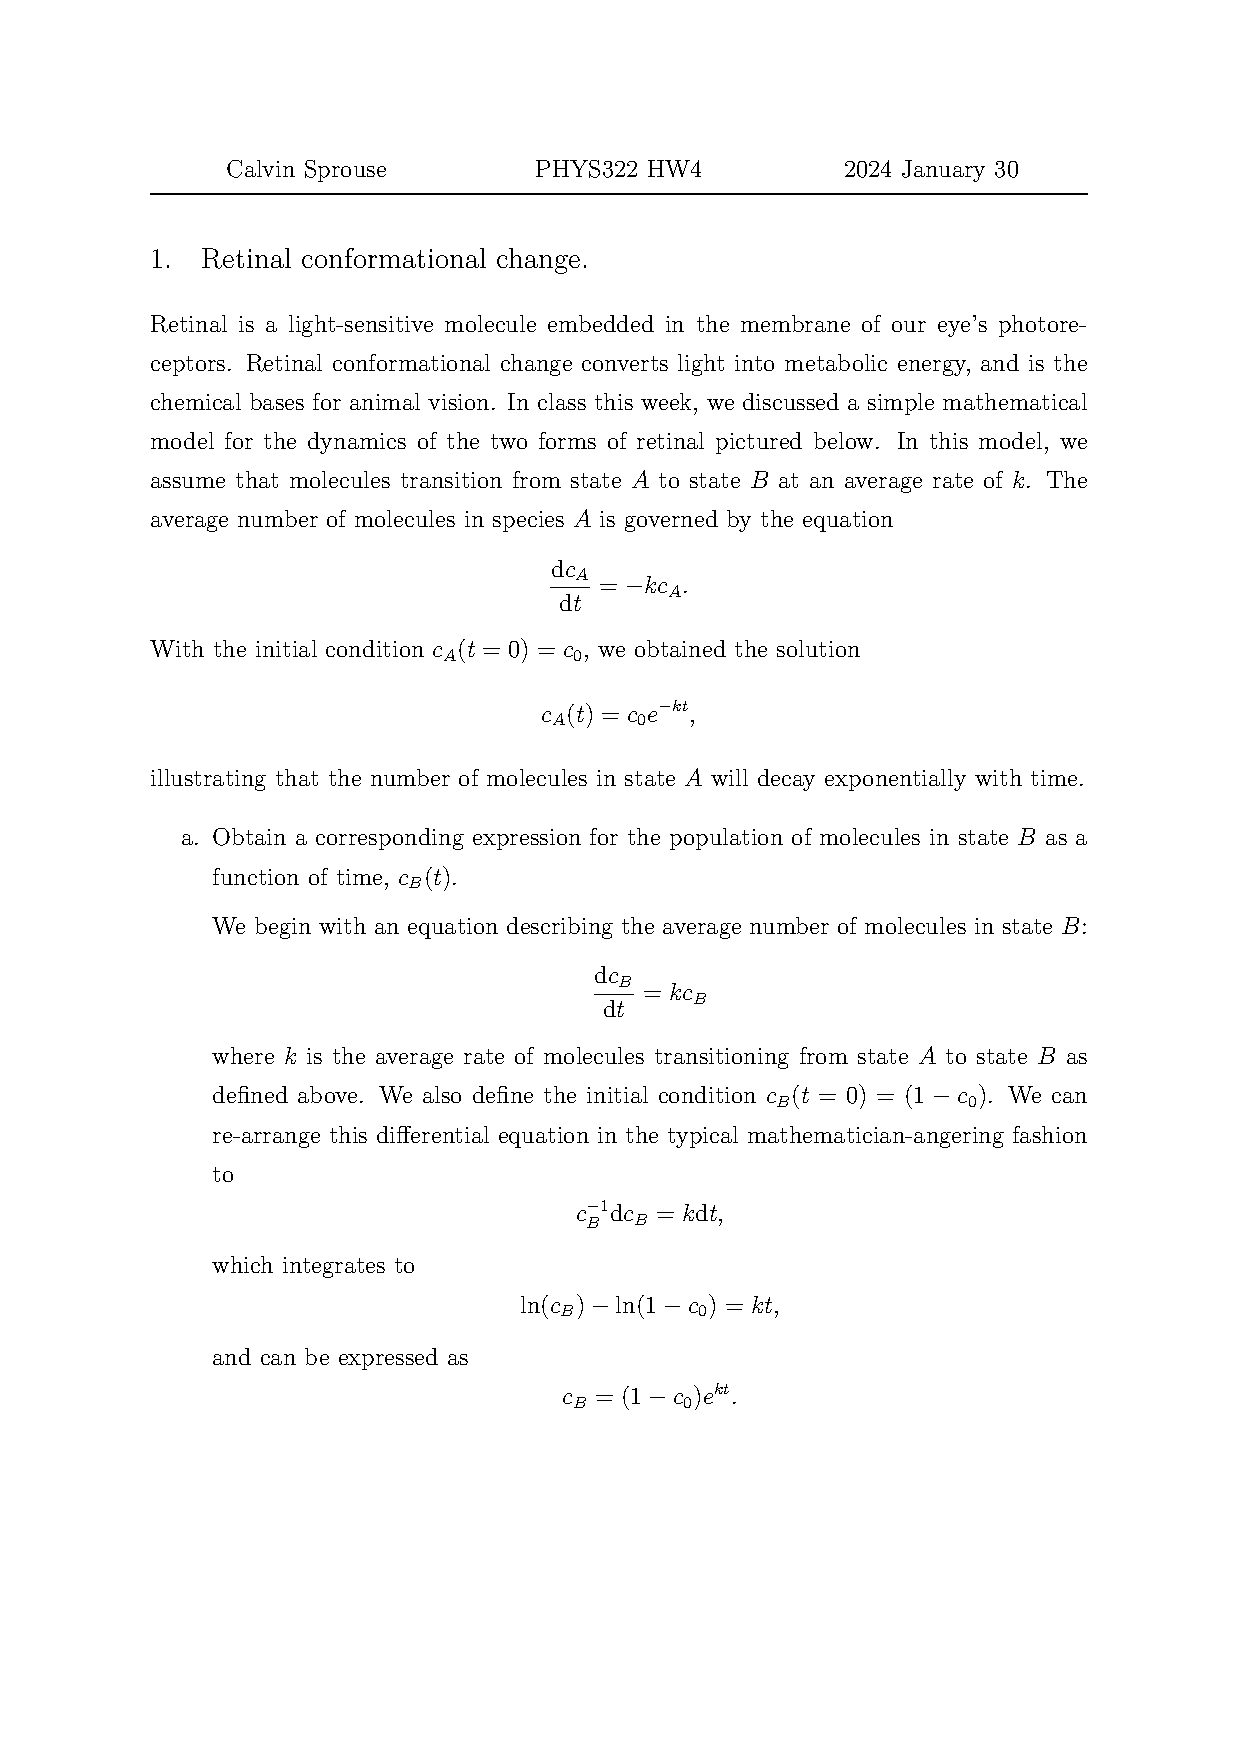
\includepdf[pages=-]{hw4.pdf}

\end{document}
